\section{Implementierung digitaler Regler}

Heutzutags werden fast nur noch digitale Regler implementiert. Gründe hierfür sind:

\begin{itemize}
    \item Verarbeitung digitaler Signale ist flexibel
    \item Speichung und Übertragung digitaler Signale ist einfach
    \item Komponenten (Rechner, Wandler) für ditigale Umsetzung werden immer günstiger
\end{itemize}


\subsection{Aufbau digitaler Regelkreis}{183}

\begin{minipage}[c]{0.63\columnwidth}
    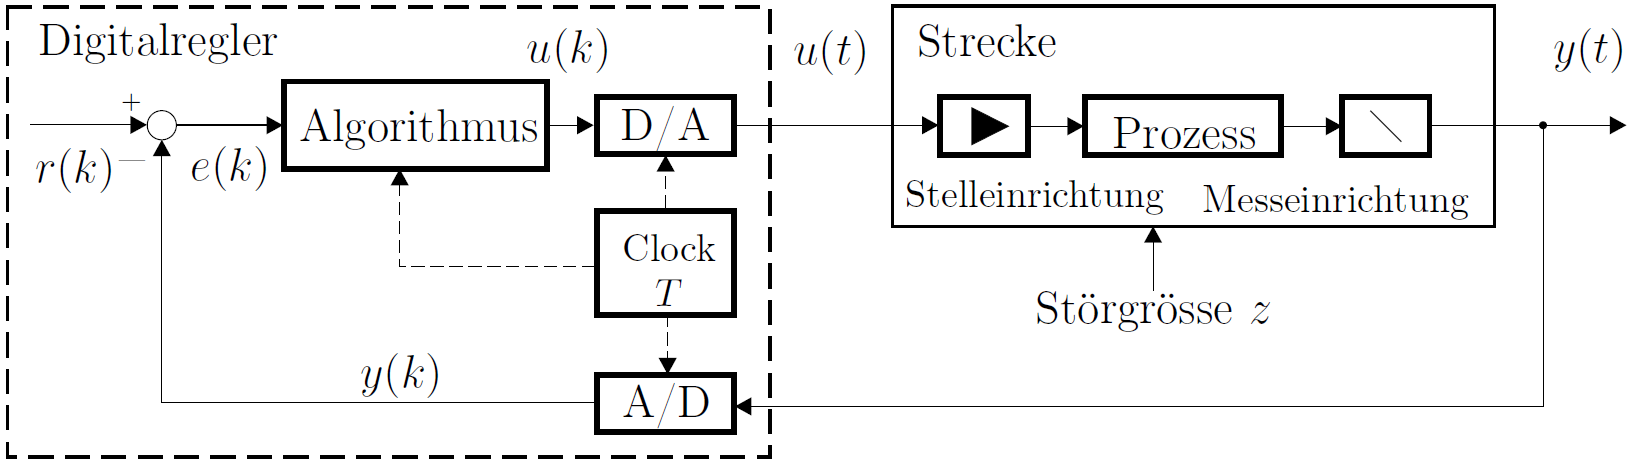
\includegraphics[width=\columnwidth]{images/regelkreis_mit_digitalregler.png}
\end{minipage}
\hfill
\begin{minipage}[c]{0.35\columnwidth}
    \begin{itemize}
        \item Strecke ändert nicht
        \item Regler arbeitet \textbf{zeitdiskret}
    \end{itemize}
\end{minipage}


\subsubsection{Signale im digitalen Regelkreis}{184}

\begin{center}
    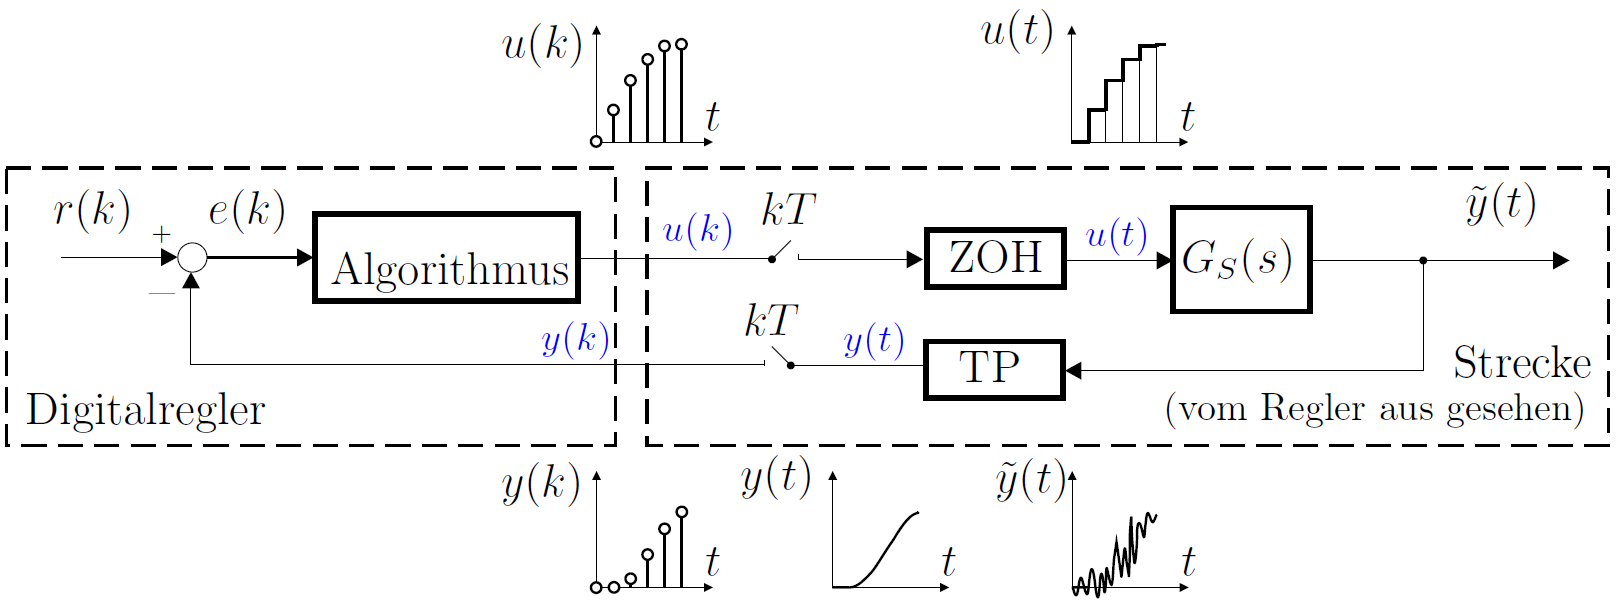
\includegraphics[width=0.75\columnwidth]{images/digitaler_regelkreis_signaltypen.png}
\end{center}

\begin{outline}
    \1 Sensorseitig wird periodisch die Regelgrösse abgetastet (zuvor TP-filtern)
        \2 \textbf{TP:} Analoges Tiefpassfilter \textrightarrow\ Anti-Aliasing
    \1 Aktorseitig wird mit \textbf{ZOH}-Halteglied (Zero-Order-Hold) aus dem diskreten Signal $u(k)$ eine kontinuierliche Funktion $u(t)$ erzeugt 
\end{outline}


\subsubsection{Quantisierung}{185}

Das Signal eines ditialen Reglers ist sowohl \textbf{zeitdiskret} als auch \textbf{wertdiskret}.

\medskip
\begin{minipage}[c]{0.49\columnwidth}
    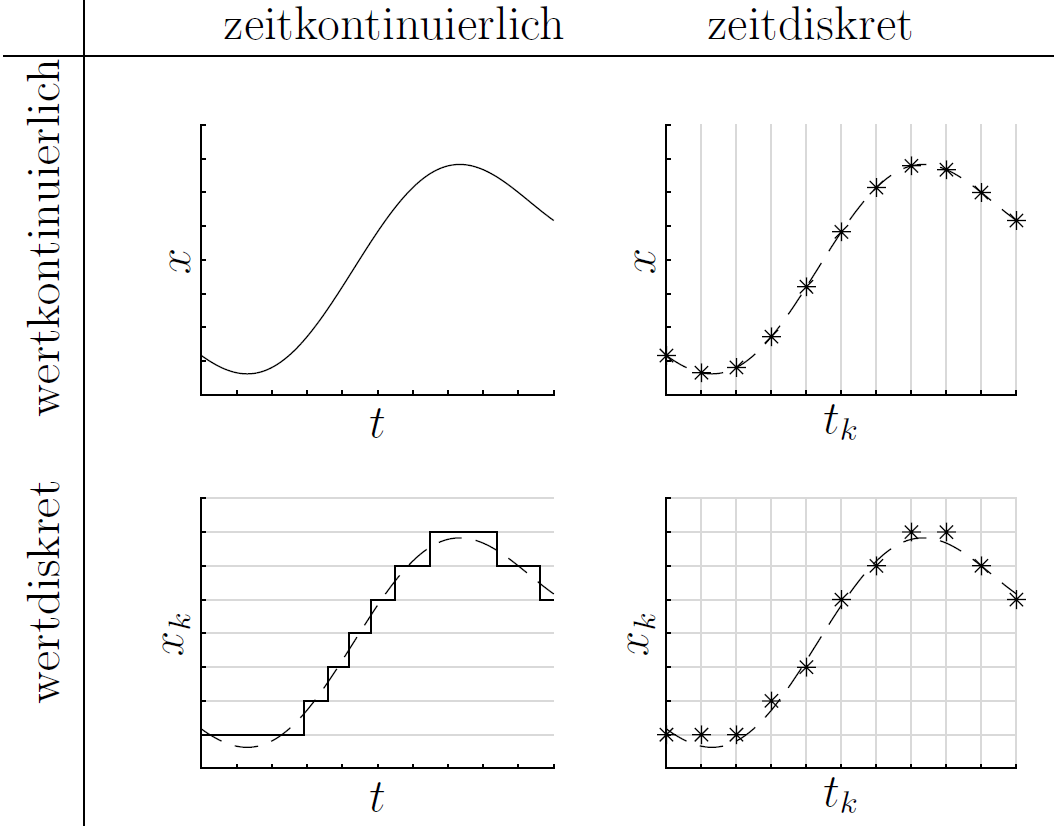
\includegraphics[width=\columnwidth]{images/abtastung.png}
\end{minipage}
\hfill
\begin{minipage}[c]{0.5\columnwidth}
    \raggedright%
    \textbf{\myul{Abtastzeit $T$}}

    \begin{outline}
        \1 $T$ zu gross gewählt
            \2 Schlechtes Führungsverhalten (Überschwingen)
        \1 $T$ zu klein gewählt
            \2 Möglicherweise numerische Probleme
            \2 Höhere Anforderungen an Sensor, Aktor, Wandler und Digitalrechner
    \end{outline}


    \textbf{\myul{Sättigung und Quantisierung}}

    \begin{outline}
        \1 Grobe Quantisierung
            \2 Nichtlineare Reglerung
        \1 Feine Quantisierung
            \2 Keinen (negativen) Einfluss auf Regler 
    \end{outline}
\end{minipage}


\subsection{Entwurfsverfahren}{186}

\begin{minipage}[c]{0.45\columnwidth}
    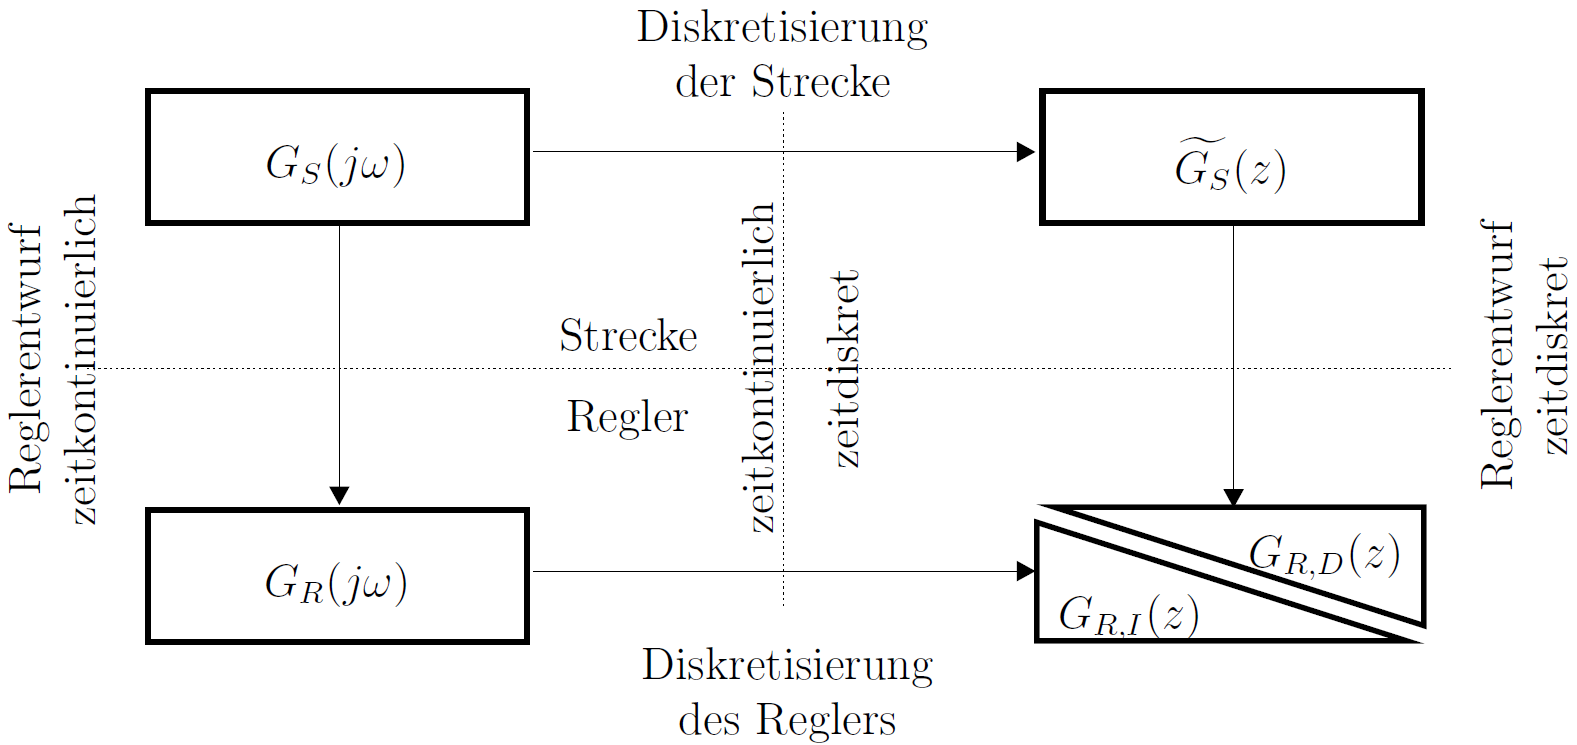
\includegraphics[width=\columnwidth]{images/direkter_indirekter_reglerentwurf_digital.png}  
\end{minipage}
\hfill
\begin{minipage}[c]{0.53\columnwidth}
    \begin{outline}
        \1  \textbf{Indirekter digitaler Reglerentwurf}
            \2 $G_S(\jimg \omega)$ \textrightarrow\ 'links herum' \textrightarrow\ $G_{R,I}(z)$
        \1 Direkter digitaler Reglerentwurf
            \2 $G_S(\jimg \omega)$ \textrightarrow\ 'rechts herum' \textrightarrow\ $G_{R,D}(z)$
            \2 'Digitale Natur' des Reglers von Anfang an berücksichtigt
    \end{outline}
\end{minipage}

\textbf{Hinweis:} Normalerweise sind die resultierenden Regler nicht identisch: $G_{R,I}(z) \neq G_{R,D}(z)$


\subsection{Diskretisierung eines Reglers}{188}

Ein kontinuierlicher Regler (hier I-Regler) weist folgendes Verhalten auf:
$$ u(t) = K_R \cdot \int\limits_0^t e(\tau) \, \diff \tau $$

Der entsprechende zeitdiskrete Regler kann \textbf{nicht exakt} gebildet werden, da $e(t)$ nur zu diskreten Zeitpunkten $e(kT)$ bekannt ist.
Geht man davon aus, dass $e(t)$ \textbf{nicht stakt ändert} (\textrightarrow\ geeignete Wahl der Abtastzeit $T$), dann kann $u(k)$
folgendermassen approximiert werden:

$$ u(k) = K_R \cdot \int\limits_0^{kT} e(\tau) \, \diff \tau
    = \underbrace{K_R \cdot \int\limits_0^{kT- T} e(\tau) \, \diff \tau}_{u(k-1)} 
    + \underbrace{K_R \cdot \int\limits_{kT-T}^{kT} e(\tau) \, \diff \tau}_{\approx A} $$


\subsubsection{Approximationen der Fläche $A$}

Die Fläche $A$ kann auf mehrere Arten approximiert werden:


\begin{minipage}[c]{0.3\columnwidth}
    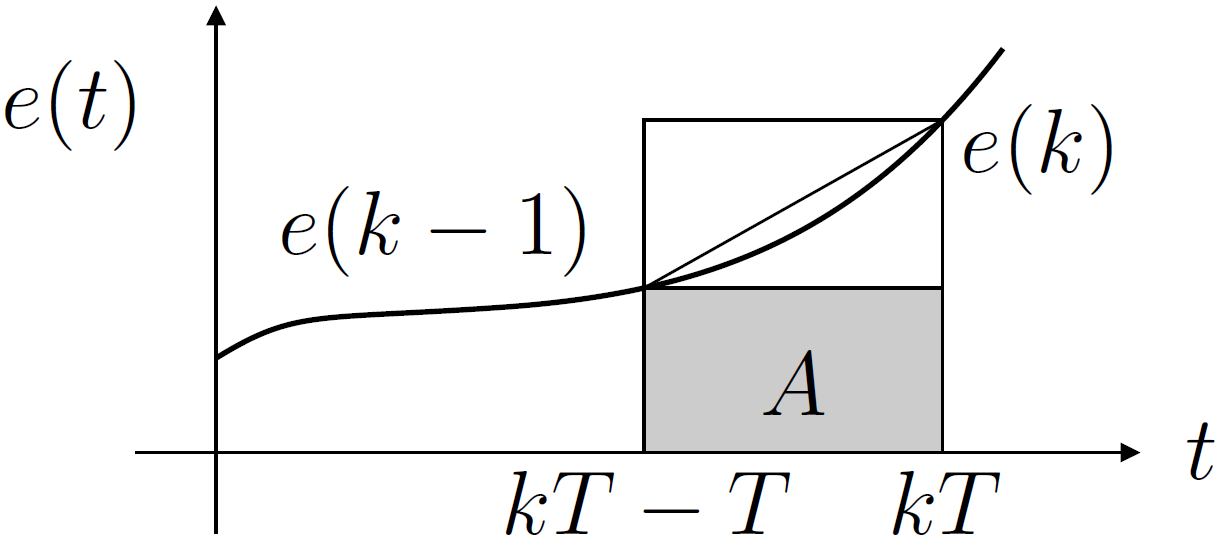
\includegraphics[width=\columnwidth]{images/approximation_integration.png}
\end{minipage}
\hfill
\begin{minipage}[c]{0.68\columnwidth}
    \begin{tabular}{ll}
        Rechteckregel vorwärts (Euler)      & $ A = T \cdot e(k-1) $    \\
        Rechteckregel rückwärts             & $ A = T \cdot e(k)$       \\
        \textbf{Trapezregel (Tustin)}       & $ A = T \cdot \frac{e(k-1) + e(k)}{1} $ 
    \end{tabular}
\end{minipage}

\vspace{0.2cm}
\textbf{Hinweis:} Für die Diskretisierung von Reglern wird die \textbf{Trapez-Approximation} verwendet, da diese am genausten ist.


\subsection{Vorgehen: Diskretisierung eines Reglers}

\begin{enumerate}
    \item Übertragungsfunktion des Reglers in $\jimg \omega$ aufstellen: $G_R(\jimg \omega) = ...$
    \item Wahl der Abtastzeit $T_S$ und einer Diskretisierungsmethode \\
        -- (typischerweise Tustin, weil am genausten)
    \item Substitution aller $\jimg \omega$ in der UTF durch Approximation in $z^{-1}$ \textrightarrow\ $G_{R, \, \rm diskret}(z) = ...$ \\
        -- Tustin: $\jimg \omega = \frac{2}{T} \frac{1 - z^{-1}}{1 + z^{-1}}$
    \item Umformen, damit Doppelbrüche verschwinden
    \item Ansatz: $G_{R, \, \rm diskret}(z) = \frac{U(z)}{E(z)}$ sortieren nach $U(z)$ und $E(z)$
    \item Differenzengleichung durch inverse Z-Transformation bestimmen
\end{enumerate}


\example{PI-Regler diskretisieren}

Gegeben sei die Übertragungsfunktion $G_R(\jimg \omega)$ eines \textbf{kontinuierlichen} Reglers.
Daraus soll die zu implementierende \textbf{Differenzengleichung} ermittelt werden.

$$ 1. \quad G_R(\jimg \omega) = K_R \cdot \frac{1 + T_N \jimg \omega}{T_N \jimg \omega} \quad {\textrightarrow\ }2. $$
$$ G_{R, \, \rm diskret}(z) \overset{3.}{=} K_R \cdot \frac{1 + T_N \frac{2}{T} \frac{1- z^{-1}}{1 + z^{-1}}}{T_N \frac{2}{T} \frac{1- z^{-1}}{1 + z^{-1}}} 
\overset{4.}{=} K_R \cdot \frac{T (1 + z^{-1}) + 2 T_N (1 - z^{-1})}{2 T_N (1- z^{-1})} = \frac{U(z)}{E(z)} $$
$$  5. \quad U(z) (1 - z^{-1}) = \frac{K_R}{2 T_N} \cdot E(z) \left\lgroup T (1 + z^{-1}) + 2 T_N (1 - z^{-1}) \right\rgroup $$
$$  6. \quad u(k) - u(k-1) = \frac{K_R}{2 T_N} \Big[ T \cdot e(k) + T \cdot e(k-1) + 2 T_N \cdot e(k) - 2 T_N \cdot e(k-1) \Big] $$
$$ u(k) = u(k-1) + \frac{K_R}{2 T_N} \Big[ e(k) \cdot \big( T + 2 T_N  \big) +  e(k-1) \cdot \big( T - 2 T_N  \big)  \Big]  $$


\subsection{Code-Implementierung eines diskreten Reglers}{190}

\lstinputlisting{snippets/digitale_regler.m}


\subsubsection{Optimierung des Speicherplatzes}{189}

\begin{minipage}[c]{0.6\columnwidth}
     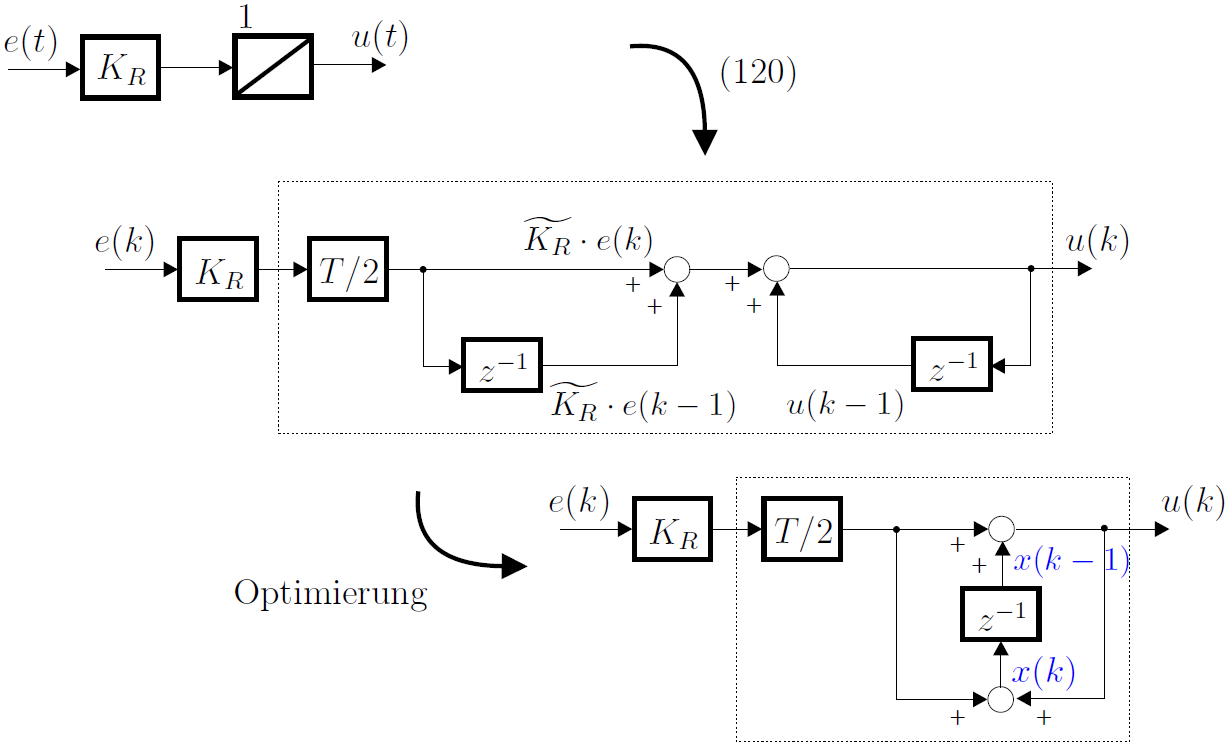
\includegraphics[width=\columnwidth]{images/optimierung_speicherplatz.png}
\end{minipage}
\hfill
\begin{minipage}[c]{0.39\columnwidth}
    Durch geeignete Anpassung kann die Struktur des Reglers so optimiert werden, dass man sich nicht mehr die beiden Werte $u(k-1)$ und $e(k-1)$
    'merken' muss, sondern nur noch einen Wert $x(k-1)$
\end{minipage}

